\documentclass[twoside]{book}

% Packages required by doxygen
\usepackage{fixltx2e}
\usepackage{calc}
\usepackage{doxygen}
\usepackage{graphicx}
\usepackage[utf8]{inputenc}
\usepackage{makeidx}
\usepackage{multicol}
\usepackage{multirow}
\PassOptionsToPackage{warn}{textcomp}
\usepackage{textcomp}
\usepackage[nointegrals]{wasysym}
\usepackage[table]{xcolor}

% Font selection
\usepackage[T1]{fontenc}
\usepackage{mathptmx}
\usepackage[scaled=.90]{helvet}
\usepackage{courier}
\usepackage{amssymb}
\usepackage{sectsty}
\renewcommand{\familydefault}{\sfdefault}
\allsectionsfont{%
  \fontseries{bc}\selectfont%
  \color{darkgray}%
}
\renewcommand{\DoxyLabelFont}{%
  \fontseries{bc}\selectfont%
  \color{darkgray}%
}
\newcommand{\+}{\discretionary{\mbox{\scriptsize$\hookleftarrow$}}{}{}}

% Page & text layout
\usepackage{geometry}
\geometry{%
  a4paper,%
  top=2.5cm,%
  bottom=2.5cm,%
  left=2.5cm,%
  right=2.5cm%
}
\tolerance=750
\hfuzz=15pt
\hbadness=750
\setlength{\emergencystretch}{15pt}
\setlength{\parindent}{0cm}
\setlength{\parskip}{0.2cm}
\makeatletter
\renewcommand{\paragraph}{%
  \@startsection{paragraph}{4}{0ex}{-1.0ex}{1.0ex}{%
    \normalfont\normalsize\bfseries\SS@parafont%
  }%
}
\renewcommand{\subparagraph}{%
  \@startsection{subparagraph}{5}{0ex}{-1.0ex}{1.0ex}{%
    \normalfont\normalsize\bfseries\SS@subparafont%
  }%
}
\makeatother

% Headers & footers
\usepackage{fancyhdr}
\pagestyle{fancyplain}
\fancyhead[LE]{\fancyplain{}{\bfseries\thepage}}
\fancyhead[CE]{\fancyplain{}{}}
\fancyhead[RE]{\fancyplain{}{\bfseries\leftmark}}
\fancyhead[LO]{\fancyplain{}{\bfseries\rightmark}}
\fancyhead[CO]{\fancyplain{}{}}
\fancyhead[RO]{\fancyplain{}{\bfseries\thepage}}
\fancyfoot[LE]{\fancyplain{}{}}
\fancyfoot[CE]{\fancyplain{}{}}
\fancyfoot[RE]{\fancyplain{}{\bfseries\scriptsize Generated on Sun Nov 9 2014 00\+:50\+:54 for Wreck by Doxygen }}
\fancyfoot[LO]{\fancyplain{}{\bfseries\scriptsize Generated on Sun Nov 9 2014 00\+:50\+:54 for Wreck by Doxygen }}
\fancyfoot[CO]{\fancyplain{}{}}
\fancyfoot[RO]{\fancyplain{}{}}
\renewcommand{\footrulewidth}{0.4pt}
\renewcommand{\chaptermark}[1]{%
  \markboth{#1}{}%
}
\renewcommand{\sectionmark}[1]{%
  \markright{\thesection\ #1}%
}

% Indices & bibliography
\usepackage{natbib}
\usepackage[titles]{tocloft}
\setcounter{tocdepth}{3}
\setcounter{secnumdepth}{5}
\makeindex

% Hyperlinks (required, but should be loaded last)
\usepackage{ifpdf}
\ifpdf
  \usepackage[pdftex,pagebackref=true]{hyperref}
\else
  \usepackage[ps2pdf,pagebackref=true]{hyperref}
\fi
\hypersetup{%
  colorlinks=true,%
  linkcolor=blue,%
  citecolor=blue,%
  unicode%
}

% Custom commands
\newcommand{\clearemptydoublepage}{%
  \newpage{\pagestyle{empty}\cleardoublepage}%
}


%===== C O N T E N T S =====

\begin{document}

% Titlepage & ToC
\hypersetup{pageanchor=false,
             bookmarks=true,
             bookmarksnumbered=true,
             pdfencoding=unicode
            }
\pagenumbering{roman}
\begin{titlepage}
\vspace*{7cm}
\begin{center}%
{\Large Wreck }\\
\vspace*{1cm}
{\large Generated by Doxygen 1.8.8}\\
\vspace*{0.5cm}
{\small Sun Nov 9 2014 00:50:54}\\
\end{center}
\end{titlepage}
\clearemptydoublepage
\tableofcontents
\clearemptydoublepage
\pagenumbering{arabic}
\hypersetup{pageanchor=true}

%--- Begin generated contents ---
\chapter{Namespace Index}
\section{Namespace List}
Here is a list of all namespaces with brief descriptions\+:\begin{DoxyCompactList}
\item\contentsline{section}{\hyperlink{namespaceoctet}{octet} }{\pageref{namespaceoctet}}{}
\end{DoxyCompactList}

\chapter{Hierarchical Index}
\section{Class Hierarchy}
This inheritance list is sorted roughly, but not completely, alphabetically\+:\begin{DoxyCompactList}
\item app\begin{DoxyCompactList}
\item \contentsline{section}{octet\+:\+:wreck\+\_\+game}{\pageref{classoctet_1_1wreck__game}}{}
\end{DoxyCompactList}
\item resource\begin{DoxyCompactList}
\item \contentsline{section}{octet\+:\+:race\+\_\+track}{\pageref{classoctet_1_1race__track}}{}
\item \contentsline{section}{octet\+:\+:vehicle}{\pageref{classoctet_1_1vehicle}}{}
\item \contentsline{section}{octet\+:\+:xbox\+\_\+controller}{\pageref{classoctet_1_1xbox__controller}}{}
\end{DoxyCompactList}
\end{DoxyCompactList}

\chapter{Class Index}
\section{Class List}
Here are the classes, structs, unions and interfaces with brief descriptions\+:\begin{DoxyCompactList}
\item\contentsline{section}{\hyperlink{classoctet_1_1race__track}{octet\+::race\+\_\+track} \\*Class for creating a race track with rigid bodies reading a .txt file }{\pageref{classoctet_1_1race__track}}{}
\item\contentsline{section}{\hyperlink{classoctet_1_1vehicle}{octet\+::vehicle} \\*Class to create a vehicle using hinges }{\pageref{classoctet_1_1vehicle}}{}
\item\contentsline{section}{\hyperlink{classoctet_1_1wreck__game}{octet\+::wreck\+\_\+game} \\*Scene using bullet for physics effects }{\pageref{classoctet_1_1wreck__game}}{}
\item\contentsline{section}{\hyperlink{classoctet_1_1xbox__controller}{octet\+::xbox\+\_\+controller} \\*Class for getting the input from an Xbox controller }{\pageref{classoctet_1_1xbox__controller}}{}
\end{DoxyCompactList}

\chapter{File Index}
\section{File List}
Here is a list of all files with brief descriptions\+:\begin{DoxyCompactList}
\item\contentsline{section}{C\+:/\+Projects/\+Wreck/octet/octet/src/examples/\+Wreck/\hyperlink{main_8cpp}{main.\+cpp} }{\pageref{main_8cpp}}{}
\item\contentsline{section}{C\+:/\+Projects/\+Wreck/octet/octet/src/examples/\+Wreck/\hyperlink{race__track_8h}{race\+\_\+track.\+h} }{\pageref{race__track_8h}}{}
\item\contentsline{section}{C\+:/\+Projects/\+Wreck/octet/octet/src/examples/\+Wreck/\hyperlink{vehicle_8h}{vehicle.\+h} }{\pageref{vehicle_8h}}{}
\item\contentsline{section}{C\+:/\+Projects/\+Wreck/octet/octet/src/examples/\+Wreck/\hyperlink{wreck__game_8h}{wreck\+\_\+game.\+h} }{\pageref{wreck__game_8h}}{}
\item\contentsline{section}{C\+:/\+Projects/\+Wreck/octet/octet/src/examples/\+Wreck/\hyperlink{xbox__controller_8h}{xbox\+\_\+controller.\+h} }{\pageref{xbox__controller_8h}}{}
\end{DoxyCompactList}

\chapter{Namespace Documentation}
\hypertarget{namespaceoctet}{\section{octet Namespace Reference}
\label{namespaceoctet}\index{octet@{octet}}
}
\subsection*{Classes}
\begin{DoxyCompactItemize}
\item 
class \hyperlink{classoctet_1_1race__track}{race\+\_\+track}
\begin{DoxyCompactList}\small\item\em Class for creating a race track with rigid bodies reading a .txt file. \end{DoxyCompactList}\item 
class \hyperlink{classoctet_1_1vehicle}{vehicle}
\begin{DoxyCompactList}\small\item\em Class to create a vehicle using hinge constraints. \end{DoxyCompactList}\item 
class \hyperlink{classoctet_1_1wreck__game}{wreck\+\_\+game}
\begin{DoxyCompactList}\small\item\em Scene using bullet for physics effects. \end{DoxyCompactList}\item 
class \hyperlink{classoctet_1_1xbox__controller}{xbox\+\_\+controller}
\begin{DoxyCompactList}\small\item\em Class for getting the input from an Xbox controller. \end{DoxyCompactList}\end{DoxyCompactItemize}

\chapter{Class Documentation}
\hypertarget{classoctet_1_1race__track}{\section{octet\+:\+:race\+\_\+track Class Reference}
\label{classoctet_1_1race__track}\index{octet\+::race\+\_\+track@{octet\+::race\+\_\+track}}
}


Class for creating a race track with rigid bodies reading a .txt file.  




{\ttfamily \#include $<$race\+\_\+track.\+h$>$}

Inheritance diagram for octet\+:\+:race\+\_\+track\+:\begin{figure}[H]
\begin{center}
\leavevmode
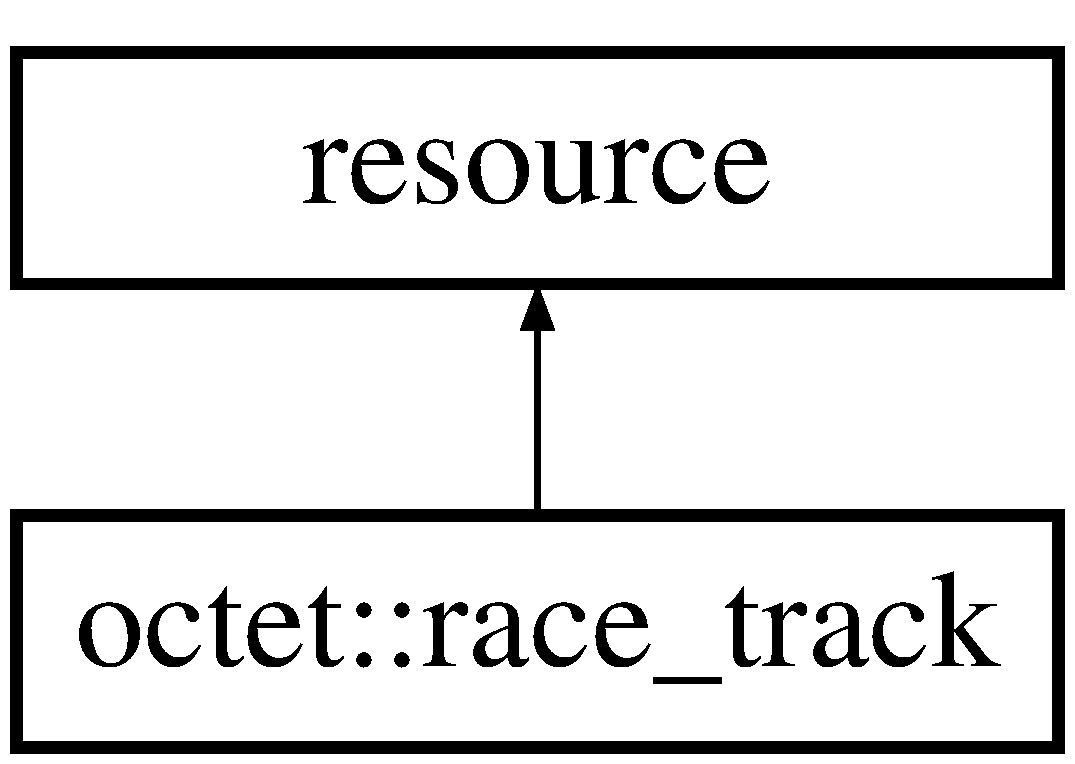
\includegraphics[height=2.000000cm]{classoctet_1_1race__track}
\end{center}
\end{figure}
\subsection*{Public Member Functions}
\begin{DoxyCompactItemize}
\item 
\hyperlink{classoctet_1_1race__track_ac4cd9e5f3cd700178c00a09c2b21445f}{race\+\_\+track} ()
\item 
void \hyperlink{classoctet_1_1race__track_ab2c04a779a0d94e7c91895de318d1314}{create\+\_\+track\+\_\+component} (mat4t\+\_\+in track\+\_\+size, mesh $\ast$msh, material $\ast$mtl, bool is\+\_\+rigid\+\_\+body)
\begin{DoxyCompactList}\small\item\em Creates a mesh and possibly a rigid body for the environment. \end{DoxyCompactList}\item 
void \hyperlink{classoctet_1_1race__track_a3d6bf1d245f23564eb8eb3b36ac463b5}{init} (app $\ast$app, visual\+\_\+scene $\ast$app\+\_\+scene, bt\+Discrete\+Dynamics\+World $\ast$world)
\begin{DoxyCompactList}\small\item\em init the class, getting the app, app\+\_\+scene and world from the main app (\hyperlink{wreck__game_8h}{wreck\+\_\+game.\+h}) \end{DoxyCompactList}\item 
\hyperlink{classoctet_1_1race__track_a03aceb6117388e72ee9cb8da2bcdd4eb}{$\sim$race\+\_\+track} ()
\end{DoxyCompactItemize}


\subsection{Detailed Description}
Class for creating a race track with rigid bodies reading a .txt file. 

A race track is created by reading in a .txt file with 10 or 11 parameters. The first 4 parameters is the model\+To\+World rotation, the next 3 is for the translation and the last 3 assign the size of the mesh box. If an 11th parameter then change the material to a road barrier. 

\subsection{Constructor \& Destructor Documentation}
\hypertarget{classoctet_1_1race__track_ac4cd9e5f3cd700178c00a09c2b21445f}{\index{octet\+::race\+\_\+track@{octet\+::race\+\_\+track}!race\+\_\+track@{race\+\_\+track}}
\index{race\+\_\+track@{race\+\_\+track}!octet\+::race\+\_\+track@{octet\+::race\+\_\+track}}
\subsubsection[{race\+\_\+track}]{\setlength{\rightskip}{0pt plus 5cm}octet\+::race\+\_\+track\+::race\+\_\+track (
\begin{DoxyParamCaption}
{}
\end{DoxyParamCaption}
)\hspace{0.3cm}{\ttfamily [inline]}}}\label{classoctet_1_1race__track_ac4cd9e5f3cd700178c00a09c2b21445f}
\hypertarget{classoctet_1_1race__track_a03aceb6117388e72ee9cb8da2bcdd4eb}{\index{octet\+::race\+\_\+track@{octet\+::race\+\_\+track}!````~race\+\_\+track@{$\sim$race\+\_\+track}}
\index{````~race\+\_\+track@{$\sim$race\+\_\+track}!octet\+::race\+\_\+track@{octet\+::race\+\_\+track}}
\subsubsection[{$\sim$race\+\_\+track}]{\setlength{\rightskip}{0pt plus 5cm}octet\+::race\+\_\+track\+::$\sim$race\+\_\+track (
\begin{DoxyParamCaption}
{}
\end{DoxyParamCaption}
)\hspace{0.3cm}{\ttfamily [inline]}}}\label{classoctet_1_1race__track_a03aceb6117388e72ee9cb8da2bcdd4eb}


\subsection{Member Function Documentation}
\hypertarget{classoctet_1_1race__track_ab2c04a779a0d94e7c91895de318d1314}{\index{octet\+::race\+\_\+track@{octet\+::race\+\_\+track}!create\+\_\+track\+\_\+component@{create\+\_\+track\+\_\+component}}
\index{create\+\_\+track\+\_\+component@{create\+\_\+track\+\_\+component}!octet\+::race\+\_\+track@{octet\+::race\+\_\+track}}
\subsubsection[{create\+\_\+track\+\_\+component}]{\setlength{\rightskip}{0pt plus 5cm}void octet\+::race\+\_\+track\+::create\+\_\+track\+\_\+component (
\begin{DoxyParamCaption}
\item[{mat4t\+\_\+in}]{track\+\_\+size, }
\item[{mesh $\ast$}]{msh, }
\item[{material $\ast$}]{mtl, }
\item[{bool}]{is\+\_\+rigid\+\_\+body}
\end{DoxyParamCaption}
)\hspace{0.3cm}{\ttfamily [inline]}}}\label{classoctet_1_1race__track_ab2c04a779a0d94e7c91895de318d1314}


Creates a mesh and possibly a rigid body for the environment. 

Mainly used to create the race track rigid mesh and rigid bodies but also used to create a skybox mesh. \hypertarget{classoctet_1_1race__track_a3d6bf1d245f23564eb8eb3b36ac463b5}{\index{octet\+::race\+\_\+track@{octet\+::race\+\_\+track}!init@{init}}
\index{init@{init}!octet\+::race\+\_\+track@{octet\+::race\+\_\+track}}
\subsubsection[{init}]{\setlength{\rightskip}{0pt plus 5cm}void octet\+::race\+\_\+track\+::init (
\begin{DoxyParamCaption}
\item[{app $\ast$}]{app, }
\item[{visual\+\_\+scene $\ast$}]{app\+\_\+scene, }
\item[{bt\+Discrete\+Dynamics\+World $\ast$}]{world}
\end{DoxyParamCaption}
)\hspace{0.3cm}{\ttfamily [inline]}}}\label{classoctet_1_1race__track_a3d6bf1d245f23564eb8eb3b36ac463b5}


init the class, getting the app, app\+\_\+scene and world from the main app (\hyperlink{wreck__game_8h}{wreck\+\_\+game.\+h}) 



The documentation for this class was generated from the following file\+:\begin{DoxyCompactItemize}
\item 
C\+:/\+Projects/\+Wreck/octet/octet/src/examples/\+Wreck/\hyperlink{race__track_8h}{race\+\_\+track.\+h}\end{DoxyCompactItemize}

\hypertarget{classoctet_1_1vehicle}{\section{octet\+:\+:vehicle Class Reference}
\label{classoctet_1_1vehicle}\index{octet\+::vehicle@{octet\+::vehicle}}
}


Class to create a vehicle using hinges.  




{\ttfamily \#include $<$vehicle.\+h$>$}

Inheritance diagram for octet\+:\+:vehicle\+:\begin{figure}[H]
\begin{center}
\leavevmode
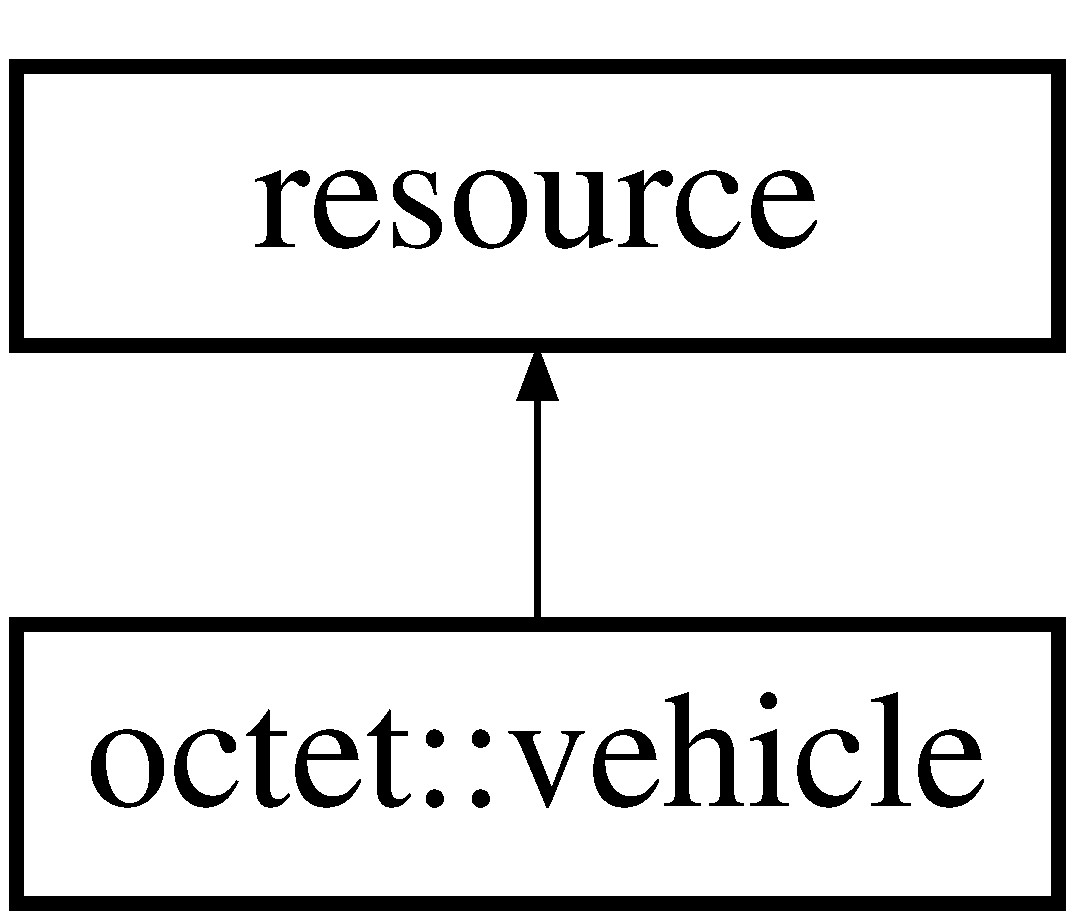
\includegraphics[height=2.000000cm]{classoctet_1_1vehicle}
\end{center}
\end{figure}
\subsection*{Public Member Functions}
\begin{DoxyCompactItemize}
\item 
\hyperlink{classoctet_1_1vehicle_a22017fec042aa7732f1699b535390787}{vehicle} ()
\item 
void \hyperlink{classoctet_1_1vehicle_aa0d5baefeba0587e62f9c62dc87506fb}{create\+\_\+car\+\_\+component} (mat4t\+\_\+in axilsize, mesh $\ast$msh, material $\ast$mtl, dynarray$<$ bt\+Rigid\+Body $\ast$ $>$ $\ast$rb\+Array, bt\+Scalar mass)
\item 
void \hyperlink{classoctet_1_1vehicle_a36bcb4433889025632bfec79f681a877}{create\+\_\+hinges} (bt\+Rigid\+Body $\ast$rb\+A, bt\+Rigid\+Body $\ast$rb\+B, dynarray$<$ bt\+Hinge\+Constraint $\ast$ $>$ $\ast$hinge\+\_\+array, vec3\+\_\+in Pivot\+A, vec3\+\_\+in Pivot\+B, vec3\+\_\+in Axis, bool set\+\_\+hinge\+\_\+limits)
\item 
void \hyperlink{classoctet_1_1vehicle_a45b69ee9ab03cf7b1c05dfdb88eb783c}{sound\+\_\+control} ()
\item 
void \hyperlink{classoctet_1_1vehicle_af1ecc8cb043d912123287e085dd3417d}{init} (app $\ast$app, visual\+\_\+scene $\ast$app\+\_\+scene, bt\+Discrete\+Dynamics\+World $\ast$world)
\item 
void \hyperlink{classoctet_1_1vehicle_a8c833c3ae603e9ae1355a60fb10a43de}{update} ()
\item 
void \hyperlink{classoctet_1_1vehicle_a21db8dc5ab149c9bd9b4243a8c7db083}{move\+\_\+direction} (float motor\+\_\+velocity, float motor\+\_\+impulse\+\_\+limit)
\item 
void \hyperlink{classoctet_1_1vehicle_a65369849e223781de684f4466074b739}{rotate\+\_\+axils} (float axil\+\_\+direction\+\_\+limit)
\item 
\hyperlink{classoctet_1_1vehicle_a8722711090082884b7f4acc4b3c2d6fe}{$\sim$vehicle} ()
\end{DoxyCompactItemize}
\subsection*{Public Attributes}
\begin{DoxyCompactItemize}
\item 
dynarray$<$ bt\+Rigid\+Body $\ast$ $>$ \hyperlink{classoctet_1_1vehicle_a86352cf9ebd9dd905ca54b5ed0767063}{wheels}
\end{DoxyCompactItemize}


\subsection{Detailed Description}
Class to create a vehicle using hinges. 

\subsection{Constructor \& Destructor Documentation}
\hypertarget{classoctet_1_1vehicle_a22017fec042aa7732f1699b535390787}{\index{octet\+::vehicle@{octet\+::vehicle}!vehicle@{vehicle}}
\index{vehicle@{vehicle}!octet\+::vehicle@{octet\+::vehicle}}
\subsubsection[{vehicle}]{\setlength{\rightskip}{0pt plus 5cm}octet\+::vehicle\+::vehicle (
\begin{DoxyParamCaption}
{}
\end{DoxyParamCaption}
)\hspace{0.3cm}{\ttfamily [inline]}}}\label{classoctet_1_1vehicle_a22017fec042aa7732f1699b535390787}
\hypertarget{classoctet_1_1vehicle_a8722711090082884b7f4acc4b3c2d6fe}{\index{octet\+::vehicle@{octet\+::vehicle}!````~vehicle@{$\sim$vehicle}}
\index{````~vehicle@{$\sim$vehicle}!octet\+::vehicle@{octet\+::vehicle}}
\subsubsection[{$\sim$vehicle}]{\setlength{\rightskip}{0pt plus 5cm}octet\+::vehicle\+::$\sim$vehicle (
\begin{DoxyParamCaption}
{}
\end{DoxyParamCaption}
)\hspace{0.3cm}{\ttfamily [inline]}}}\label{classoctet_1_1vehicle_a8722711090082884b7f4acc4b3c2d6fe}


\subsection{Member Function Documentation}
\hypertarget{classoctet_1_1vehicle_aa0d5baefeba0587e62f9c62dc87506fb}{\index{octet\+::vehicle@{octet\+::vehicle}!create\+\_\+car\+\_\+component@{create\+\_\+car\+\_\+component}}
\index{create\+\_\+car\+\_\+component@{create\+\_\+car\+\_\+component}!octet\+::vehicle@{octet\+::vehicle}}
\subsubsection[{create\+\_\+car\+\_\+component}]{\setlength{\rightskip}{0pt plus 5cm}void octet\+::vehicle\+::create\+\_\+car\+\_\+component (
\begin{DoxyParamCaption}
\item[{mat4t\+\_\+in}]{axilsize, }
\item[{mesh $\ast$}]{msh, }
\item[{material $\ast$}]{mtl, }
\item[{dynarray$<$ bt\+Rigid\+Body $\ast$ $>$ $\ast$}]{rb\+Array, }
\item[{bt\+Scalar}]{mass}
\end{DoxyParamCaption}
)\hspace{0.3cm}{\ttfamily [inline]}}}\label{classoctet_1_1vehicle_aa0d5baefeba0587e62f9c62dc87506fb}
\hypertarget{classoctet_1_1vehicle_a36bcb4433889025632bfec79f681a877}{\index{octet\+::vehicle@{octet\+::vehicle}!create\+\_\+hinges@{create\+\_\+hinges}}
\index{create\+\_\+hinges@{create\+\_\+hinges}!octet\+::vehicle@{octet\+::vehicle}}
\subsubsection[{create\+\_\+hinges}]{\setlength{\rightskip}{0pt plus 5cm}void octet\+::vehicle\+::create\+\_\+hinges (
\begin{DoxyParamCaption}
\item[{bt\+Rigid\+Body $\ast$}]{rb\+A, }
\item[{bt\+Rigid\+Body $\ast$}]{rb\+B, }
\item[{dynarray$<$ bt\+Hinge\+Constraint $\ast$ $>$ $\ast$}]{hinge\+\_\+array, }
\item[{vec3\+\_\+in}]{Pivot\+A, }
\item[{vec3\+\_\+in}]{Pivot\+B, }
\item[{vec3\+\_\+in}]{Axis, }
\item[{bool}]{set\+\_\+hinge\+\_\+limits}
\end{DoxyParamCaption}
)\hspace{0.3cm}{\ttfamily [inline]}}}\label{classoctet_1_1vehicle_a36bcb4433889025632bfec79f681a877}
\hypertarget{classoctet_1_1vehicle_af1ecc8cb043d912123287e085dd3417d}{\index{octet\+::vehicle@{octet\+::vehicle}!init@{init}}
\index{init@{init}!octet\+::vehicle@{octet\+::vehicle}}
\subsubsection[{init}]{\setlength{\rightskip}{0pt plus 5cm}void octet\+::vehicle\+::init (
\begin{DoxyParamCaption}
\item[{app $\ast$}]{app, }
\item[{visual\+\_\+scene $\ast$}]{app\+\_\+scene, }
\item[{bt\+Discrete\+Dynamics\+World $\ast$}]{world}
\end{DoxyParamCaption}
)\hspace{0.3cm}{\ttfamily [inline]}}}\label{classoctet_1_1vehicle_af1ecc8cb043d912123287e085dd3417d}
\hypertarget{classoctet_1_1vehicle_a21db8dc5ab149c9bd9b4243a8c7db083}{\index{octet\+::vehicle@{octet\+::vehicle}!move\+\_\+direction@{move\+\_\+direction}}
\index{move\+\_\+direction@{move\+\_\+direction}!octet\+::vehicle@{octet\+::vehicle}}
\subsubsection[{move\+\_\+direction}]{\setlength{\rightskip}{0pt plus 5cm}void octet\+::vehicle\+::move\+\_\+direction (
\begin{DoxyParamCaption}
\item[{float}]{motor\+\_\+velocity, }
\item[{float}]{motor\+\_\+impulse\+\_\+limit}
\end{DoxyParamCaption}
)\hspace{0.3cm}{\ttfamily [inline]}}}\label{classoctet_1_1vehicle_a21db8dc5ab149c9bd9b4243a8c7db083}
Move the vehicle by setting a velocity on the hinge angular motors. To move the vehicle, all 4 axils are activated and the angular motor on all Axil-\/\+Wheel hinge constraints are enabled. a motor velocity and a maximum impulse is then set to the hinge. \hypertarget{classoctet_1_1vehicle_a65369849e223781de684f4466074b739}{\index{octet\+::vehicle@{octet\+::vehicle}!rotate\+\_\+axils@{rotate\+\_\+axils}}
\index{rotate\+\_\+axils@{rotate\+\_\+axils}!octet\+::vehicle@{octet\+::vehicle}}
\subsubsection[{rotate\+\_\+axils}]{\setlength{\rightskip}{0pt plus 5cm}void octet\+::vehicle\+::rotate\+\_\+axils (
\begin{DoxyParamCaption}
\item[{float}]{axil\+\_\+direction\+\_\+limit}
\end{DoxyParamCaption}
)\hspace{0.3cm}{\ttfamily [inline]}}}\label{classoctet_1_1vehicle_a65369849e223781de684f4466074b739}
Function to take in the radian at which to turn the vehicle. The vehicle is turned by activating the front two axils in the scene and applying an angular rotation on the free angle in the Chassis-\/\+Axil hinge constraints \hypertarget{classoctet_1_1vehicle_a45b69ee9ab03cf7b1c05dfdb88eb783c}{\index{octet\+::vehicle@{octet\+::vehicle}!sound\+\_\+control@{sound\+\_\+control}}
\index{sound\+\_\+control@{sound\+\_\+control}!octet\+::vehicle@{octet\+::vehicle}}
\subsubsection[{sound\+\_\+control}]{\setlength{\rightskip}{0pt plus 5cm}void octet\+::vehicle\+::sound\+\_\+control (
\begin{DoxyParamCaption}
{}
\end{DoxyParamCaption}
)\hspace{0.3cm}{\ttfamily [inline]}}}\label{classoctet_1_1vehicle_a45b69ee9ab03cf7b1c05dfdb88eb783c}
Function to play sound when the vehicle is moving. sound\+\_\+control gets the source state of \hypertarget{classoctet_1_1vehicle_a8c833c3ae603e9ae1355a60fb10a43de}{\index{octet\+::vehicle@{octet\+::vehicle}!update@{update}}
\index{update@{update}!octet\+::vehicle@{octet\+::vehicle}}
\subsubsection[{update}]{\setlength{\rightskip}{0pt plus 5cm}void octet\+::vehicle\+::update (
\begin{DoxyParamCaption}
{}
\end{DoxyParamCaption}
)\hspace{0.3cm}{\ttfamily [inline]}}}\label{classoctet_1_1vehicle_a8c833c3ae603e9ae1355a60fb10a43de}
Update the vehicle class every frame, called from the main app \hyperlink{classoctet_1_1wreck__game}{wreck\+\_\+game}. Update takes care of the keyboard inputs and checks if an xbox controller has been connected. Keyboard inputs and the Xbox controller will not work together and keyboard inputs are taken as default. If an Xbox controller is found then the inputs from the xbox controller are taken instead. 

\subsection{Member Data Documentation}
\hypertarget{classoctet_1_1vehicle_a86352cf9ebd9dd905ca54b5ed0767063}{\index{octet\+::vehicle@{octet\+::vehicle}!wheels@{wheels}}
\index{wheels@{wheels}!octet\+::vehicle@{octet\+::vehicle}}
\subsubsection[{wheels}]{\setlength{\rightskip}{0pt plus 5cm}dynarray$<$bt\+Rigid\+Body$\ast$$>$ octet\+::vehicle\+::wheels}}\label{classoctet_1_1vehicle_a86352cf9ebd9dd905ca54b5ed0767063}


The documentation for this class was generated from the following file\+:\begin{DoxyCompactItemize}
\item 
C\+:/\+Projects/\+Wreck/octet/octet/src/examples/\+Wreck/\hyperlink{vehicle_8h}{vehicle.\+h}\end{DoxyCompactItemize}

\hypertarget{classoctet_1_1wreck__game}{\section{octet\+:\+:wreck\+\_\+game Class Reference}
\label{classoctet_1_1wreck__game}\index{octet\+::wreck\+\_\+game@{octet\+::wreck\+\_\+game}}
}


Scene using bullet for physics effects.  




{\ttfamily \#include $<$wreck\+\_\+game.\+h$>$}

Inheritance diagram for octet\+:\+:wreck\+\_\+game\+:\begin{figure}[H]
\begin{center}
\leavevmode
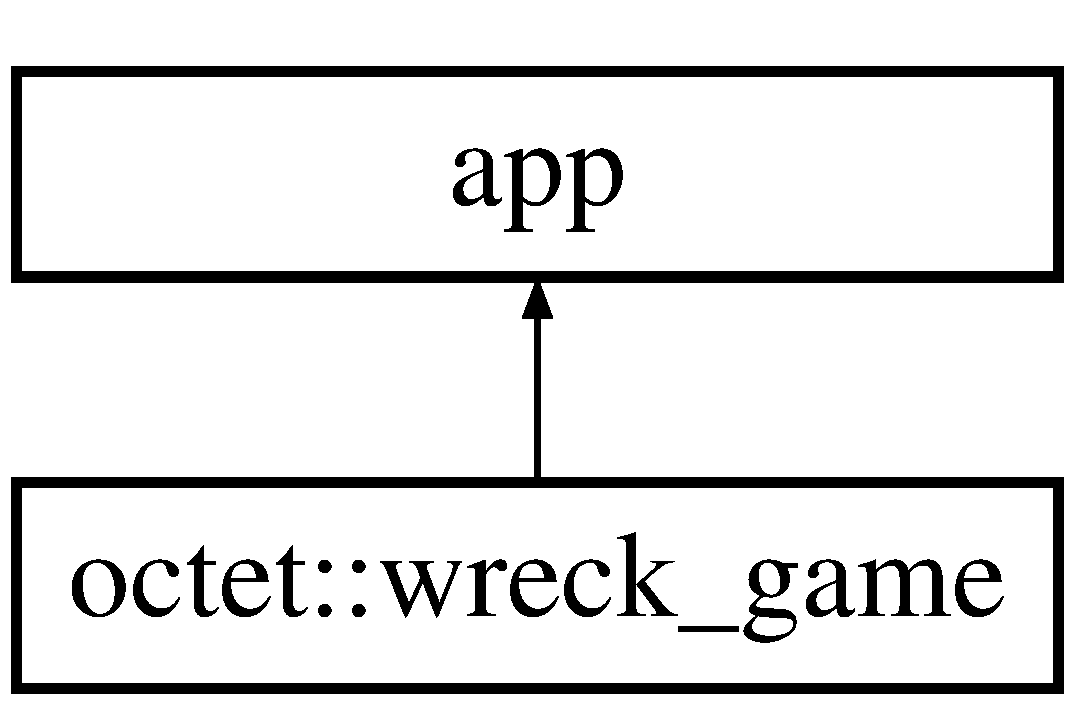
\includegraphics[height=2.000000cm]{classoctet_1_1wreck__game}
\end{center}
\end{figure}
\subsection*{Public Member Functions}
\begin{DoxyCompactItemize}
\item 
\hyperlink{classoctet_1_1wreck__game_a3415715222482226f53af7aacc322086}{wreck\+\_\+game} (int argc, char $\ast$$\ast$argv)
\begin{DoxyCompactList}\small\item\em this is called when we construct the class before everything is initialised. \end{DoxyCompactList}\item 
\hyperlink{classoctet_1_1wreck__game_aa9331cd36dbb1205931d048057061e14}{$\sim$wreck\+\_\+game} ()
\item 
void \hyperlink{classoctet_1_1wreck__game_a37f0e2212d11669e135ea848970222b5}{app\+\_\+init} ()
\begin{DoxyCompactList}\small\item\em this is called once Open\+G\+L is initialized \end{DoxyCompactList}\item 
void \hyperlink{classoctet_1_1wreck__game_a43318fc0804e69cf356cc5d35d942a66}{draw\+\_\+world} (int x, int y, int w, int h)
\begin{DoxyCompactList}\small\item\em this is called to draw the world \end{DoxyCompactList}\end{DoxyCompactItemize}


\subsection{Detailed Description}
Scene using bullet for physics effects. 

\subsection{Constructor \& Destructor Documentation}
\hypertarget{classoctet_1_1wreck__game_a3415715222482226f53af7aacc322086}{\index{octet\+::wreck\+\_\+game@{octet\+::wreck\+\_\+game}!wreck\+\_\+game@{wreck\+\_\+game}}
\index{wreck\+\_\+game@{wreck\+\_\+game}!octet\+::wreck\+\_\+game@{octet\+::wreck\+\_\+game}}
\subsubsection[{wreck\+\_\+game}]{\setlength{\rightskip}{0pt plus 5cm}octet\+::wreck\+\_\+game\+::wreck\+\_\+game (
\begin{DoxyParamCaption}
\item[{int}]{argc, }
\item[{char $\ast$$\ast$}]{argv}
\end{DoxyParamCaption}
)\hspace{0.3cm}{\ttfamily [inline]}}}\label{classoctet_1_1wreck__game_a3415715222482226f53af7aacc322086}


this is called when we construct the class before everything is initialised. 

\hypertarget{classoctet_1_1wreck__game_aa9331cd36dbb1205931d048057061e14}{\index{octet\+::wreck\+\_\+game@{octet\+::wreck\+\_\+game}!````~wreck\+\_\+game@{$\sim$wreck\+\_\+game}}
\index{````~wreck\+\_\+game@{$\sim$wreck\+\_\+game}!octet\+::wreck\+\_\+game@{octet\+::wreck\+\_\+game}}
\subsubsection[{$\sim$wreck\+\_\+game}]{\setlength{\rightskip}{0pt plus 5cm}octet\+::wreck\+\_\+game\+::$\sim$wreck\+\_\+game (
\begin{DoxyParamCaption}
{}
\end{DoxyParamCaption}
)\hspace{0.3cm}{\ttfamily [inline]}}}\label{classoctet_1_1wreck__game_aa9331cd36dbb1205931d048057061e14}


\subsection{Member Function Documentation}
\hypertarget{classoctet_1_1wreck__game_a37f0e2212d11669e135ea848970222b5}{\index{octet\+::wreck\+\_\+game@{octet\+::wreck\+\_\+game}!app\+\_\+init@{app\+\_\+init}}
\index{app\+\_\+init@{app\+\_\+init}!octet\+::wreck\+\_\+game@{octet\+::wreck\+\_\+game}}
\subsubsection[{app\+\_\+init}]{\setlength{\rightskip}{0pt plus 5cm}void octet\+::wreck\+\_\+game\+::app\+\_\+init (
\begin{DoxyParamCaption}
{}
\end{DoxyParamCaption}
)\hspace{0.3cm}{\ttfamily [inline]}}}\label{classoctet_1_1wreck__game_a37f0e2212d11669e135ea848970222b5}


this is called once Open\+G\+L is initialized 

\hypertarget{classoctet_1_1wreck__game_a43318fc0804e69cf356cc5d35d942a66}{\index{octet\+::wreck\+\_\+game@{octet\+::wreck\+\_\+game}!draw\+\_\+world@{draw\+\_\+world}}
\index{draw\+\_\+world@{draw\+\_\+world}!octet\+::wreck\+\_\+game@{octet\+::wreck\+\_\+game}}
\subsubsection[{draw\+\_\+world}]{\setlength{\rightskip}{0pt plus 5cm}void octet\+::wreck\+\_\+game\+::draw\+\_\+world (
\begin{DoxyParamCaption}
\item[{int}]{x, }
\item[{int}]{y, }
\item[{int}]{w, }
\item[{int}]{h}
\end{DoxyParamCaption}
)\hspace{0.3cm}{\ttfamily [inline]}}}\label{classoctet_1_1wreck__game_a43318fc0804e69cf356cc5d35d942a66}


this is called to draw the world 



The documentation for this class was generated from the following file\+:\begin{DoxyCompactItemize}
\item 
C\+:/\+Projects/\+Wreck/octet/octet/src/examples/\+Wreck/\hyperlink{wreck__game_8h}{wreck\+\_\+game.\+h}\end{DoxyCompactItemize}

\hypertarget{classoctet_1_1xbox__controller}{\section{octet\+:\+:xbox\+\_\+controller Class Reference}
\label{classoctet_1_1xbox__controller}\index{octet\+::xbox\+\_\+controller@{octet\+::xbox\+\_\+controller}}
}


Class for getting the input from an Xbox controller.  




{\ttfamily \#include $<$xbox\+\_\+controller.\+h$>$}

Inheritance diagram for octet\+:\+:xbox\+\_\+controller\+:\begin{figure}[H]
\begin{center}
\leavevmode
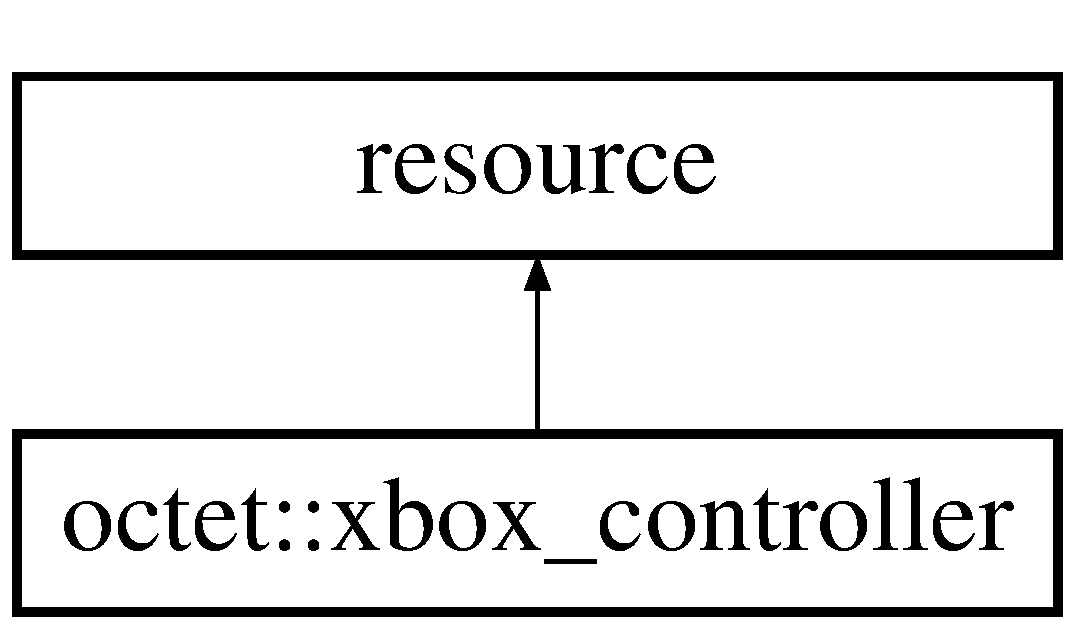
\includegraphics[height=2.000000cm]{classoctet_1_1xbox__controller}
\end{center}
\end{figure}
\subsection*{Public Member Functions}
\begin{DoxyCompactItemize}
\item 
\hyperlink{classoctet_1_1xbox__controller_a23dae5b93d48b45fee3d992b1afed77b}{xbox\+\_\+controller} ()
\item 
X\+I\+N\+P\+U\+T\+\_\+\+G\+A\+M\+E\+P\+A\+D $\ast$ \hyperlink{classoctet_1_1xbox__controller_a3a2a6b8a5ab904bf5bbb20538a7326ce}{get\+\_\+state} ()
\begin{DoxyCompactList}\small\item\em returns the current state of the xbox controller \end{DoxyCompactList}\item 
bool \hyperlink{classoctet_1_1xbox__controller_ab6fc7aad7d4c37e56511bb87dff70459}{is\+\_\+connected} ()
\begin{DoxyCompactList}\small\item\em returns true if an xbox controller is connected, returning the id of the controller (1-\/4) \end{DoxyCompactList}\item 
float \hyperlink{classoctet_1_1xbox__controller_aaf78537caeec8411d12a39a7c2f6b90c}{map\+\_\+values} (float x, float in\+\_\+min, float in\+\_\+max, float out\+\_\+min, float out\+\_\+max)
\begin{DoxyCompactList}\small\item\em map\+\_\+values allows the mapping of two values from the xbox controller, useful for specfic desired values \end{DoxyCompactList}\item 
bool \hyperlink{classoctet_1_1xbox__controller_a374fc9fd466a1155b44432eef1179073}{analog\+\_\+deadzone} ()
\begin{DoxyCompactList}\small\item\em returns whether or not the analog values are in the deadzone \end{DoxyCompactList}\item 
bool \hyperlink{classoctet_1_1xbox__controller_afa8298b80294785c3b320ccc6c6e51bd}{refresh} ()
\begin{DoxyCompactList}\small\item\em check to see if a device is connected and updates values accordingly, returns false if device is not connected, equivalent to an update function. \end{DoxyCompactList}\end{DoxyCompactItemize}
\subsection*{Public Attributes}
\begin{DoxyCompactItemize}
\item 
float \hyperlink{classoctet_1_1xbox__controller_a1860e2290b33fa35c7b57f6ceaa78881}{left\+\_\+trigger} = 0.\+0f
\item 
float \hyperlink{classoctet_1_1xbox__controller_a8406f69ac00c5ee2107e2fbea7980cd3}{right\+\_\+trigger} = 0.\+0f
\item 
float \hyperlink{classoctet_1_1xbox__controller_a4155ad43e820b46bdc1d4bced4d232ab}{left\+\_\+analog\+\_\+x} = 0.\+0f
\item 
float \hyperlink{classoctet_1_1xbox__controller_aaa5d7e08fd31b573ad296357619284d3}{left\+\_\+analog\+\_\+y} = 0.\+0f
\end{DoxyCompactItemize}


\subsection{Detailed Description}
Class for getting the input from an Xbox controller. 

The class is called to check if an Xbox controller is connected and if it is, get various inputs from it. Currently, the only inputs that are being checked are the left trigger, right trigger and the left analog stick. 

\subsection{Constructor \& Destructor Documentation}
\hypertarget{classoctet_1_1xbox__controller_a23dae5b93d48b45fee3d992b1afed77b}{\index{octet\+::xbox\+\_\+controller@{octet\+::xbox\+\_\+controller}!xbox\+\_\+controller@{xbox\+\_\+controller}}
\index{xbox\+\_\+controller@{xbox\+\_\+controller}!octet\+::xbox\+\_\+controller@{octet\+::xbox\+\_\+controller}}
\subsubsection[{xbox\+\_\+controller}]{\setlength{\rightskip}{0pt plus 5cm}octet\+::xbox\+\_\+controller\+::xbox\+\_\+controller (
\begin{DoxyParamCaption}
{}
\end{DoxyParamCaption}
)\hspace{0.3cm}{\ttfamily [inline]}}}\label{classoctet_1_1xbox__controller_a23dae5b93d48b45fee3d992b1afed77b}


\subsection{Member Function Documentation}
\hypertarget{classoctet_1_1xbox__controller_a374fc9fd466a1155b44432eef1179073}{\index{octet\+::xbox\+\_\+controller@{octet\+::xbox\+\_\+controller}!analog\+\_\+deadzone@{analog\+\_\+deadzone}}
\index{analog\+\_\+deadzone@{analog\+\_\+deadzone}!octet\+::xbox\+\_\+controller@{octet\+::xbox\+\_\+controller}}
\subsubsection[{analog\+\_\+deadzone}]{\setlength{\rightskip}{0pt plus 5cm}bool octet\+::xbox\+\_\+controller\+::analog\+\_\+deadzone (
\begin{DoxyParamCaption}
{}
\end{DoxyParamCaption}
)\hspace{0.3cm}{\ttfamily [inline]}}}\label{classoctet_1_1xbox__controller_a374fc9fd466a1155b44432eef1179073}


returns whether or not the analog values are in the deadzone 

\hypertarget{classoctet_1_1xbox__controller_a3a2a6b8a5ab904bf5bbb20538a7326ce}{\index{octet\+::xbox\+\_\+controller@{octet\+::xbox\+\_\+controller}!get\+\_\+state@{get\+\_\+state}}
\index{get\+\_\+state@{get\+\_\+state}!octet\+::xbox\+\_\+controller@{octet\+::xbox\+\_\+controller}}
\subsubsection[{get\+\_\+state}]{\setlength{\rightskip}{0pt plus 5cm}X\+I\+N\+P\+U\+T\+\_\+\+G\+A\+M\+E\+P\+A\+D$\ast$ octet\+::xbox\+\_\+controller\+::get\+\_\+state (
\begin{DoxyParamCaption}
{}
\end{DoxyParamCaption}
)\hspace{0.3cm}{\ttfamily [inline]}}}\label{classoctet_1_1xbox__controller_a3a2a6b8a5ab904bf5bbb20538a7326ce}


returns the current state of the xbox controller 

\hypertarget{classoctet_1_1xbox__controller_ab6fc7aad7d4c37e56511bb87dff70459}{\index{octet\+::xbox\+\_\+controller@{octet\+::xbox\+\_\+controller}!is\+\_\+connected@{is\+\_\+connected}}
\index{is\+\_\+connected@{is\+\_\+connected}!octet\+::xbox\+\_\+controller@{octet\+::xbox\+\_\+controller}}
\subsubsection[{is\+\_\+connected}]{\setlength{\rightskip}{0pt plus 5cm}bool octet\+::xbox\+\_\+controller\+::is\+\_\+connected (
\begin{DoxyParamCaption}
{}
\end{DoxyParamCaption}
)\hspace{0.3cm}{\ttfamily [inline]}}}\label{classoctet_1_1xbox__controller_ab6fc7aad7d4c37e56511bb87dff70459}


returns true if an xbox controller is connected, returning the id of the controller (1-\/4) 

\hypertarget{classoctet_1_1xbox__controller_aaf78537caeec8411d12a39a7c2f6b90c}{\index{octet\+::xbox\+\_\+controller@{octet\+::xbox\+\_\+controller}!map\+\_\+values@{map\+\_\+values}}
\index{map\+\_\+values@{map\+\_\+values}!octet\+::xbox\+\_\+controller@{octet\+::xbox\+\_\+controller}}
\subsubsection[{map\+\_\+values}]{\setlength{\rightskip}{0pt plus 5cm}float octet\+::xbox\+\_\+controller\+::map\+\_\+values (
\begin{DoxyParamCaption}
\item[{float}]{x, }
\item[{float}]{in\+\_\+min, }
\item[{float}]{in\+\_\+max, }
\item[{float}]{out\+\_\+min, }
\item[{float}]{out\+\_\+max}
\end{DoxyParamCaption}
)\hspace{0.3cm}{\ttfamily [inline]}}}\label{classoctet_1_1xbox__controller_aaf78537caeec8411d12a39a7c2f6b90c}


map\+\_\+values allows the mapping of two values from the xbox controller, useful for specfic desired values 

\hypertarget{classoctet_1_1xbox__controller_afa8298b80294785c3b320ccc6c6e51bd}{\index{octet\+::xbox\+\_\+controller@{octet\+::xbox\+\_\+controller}!refresh@{refresh}}
\index{refresh@{refresh}!octet\+::xbox\+\_\+controller@{octet\+::xbox\+\_\+controller}}
\subsubsection[{refresh}]{\setlength{\rightskip}{0pt plus 5cm}bool octet\+::xbox\+\_\+controller\+::refresh (
\begin{DoxyParamCaption}
{}
\end{DoxyParamCaption}
)\hspace{0.3cm}{\ttfamily [inline]}}}\label{classoctet_1_1xbox__controller_afa8298b80294785c3b320ccc6c6e51bd}


check to see if a device is connected and updates values accordingly, returns false if device is not connected, equivalent to an update function. 



\subsection{Member Data Documentation}
\hypertarget{classoctet_1_1xbox__controller_a4155ad43e820b46bdc1d4bced4d232ab}{\index{octet\+::xbox\+\_\+controller@{octet\+::xbox\+\_\+controller}!left\+\_\+analog\+\_\+x@{left\+\_\+analog\+\_\+x}}
\index{left\+\_\+analog\+\_\+x@{left\+\_\+analog\+\_\+x}!octet\+::xbox\+\_\+controller@{octet\+::xbox\+\_\+controller}}
\subsubsection[{left\+\_\+analog\+\_\+x}]{\setlength{\rightskip}{0pt plus 5cm}float octet\+::xbox\+\_\+controller\+::left\+\_\+analog\+\_\+x = 0.\+0f}}\label{classoctet_1_1xbox__controller_a4155ad43e820b46bdc1d4bced4d232ab}
\hypertarget{classoctet_1_1xbox__controller_aaa5d7e08fd31b573ad296357619284d3}{\index{octet\+::xbox\+\_\+controller@{octet\+::xbox\+\_\+controller}!left\+\_\+analog\+\_\+y@{left\+\_\+analog\+\_\+y}}
\index{left\+\_\+analog\+\_\+y@{left\+\_\+analog\+\_\+y}!octet\+::xbox\+\_\+controller@{octet\+::xbox\+\_\+controller}}
\subsubsection[{left\+\_\+analog\+\_\+y}]{\setlength{\rightskip}{0pt plus 5cm}float octet\+::xbox\+\_\+controller\+::left\+\_\+analog\+\_\+y = 0.\+0f}}\label{classoctet_1_1xbox__controller_aaa5d7e08fd31b573ad296357619284d3}
\hypertarget{classoctet_1_1xbox__controller_a1860e2290b33fa35c7b57f6ceaa78881}{\index{octet\+::xbox\+\_\+controller@{octet\+::xbox\+\_\+controller}!left\+\_\+trigger@{left\+\_\+trigger}}
\index{left\+\_\+trigger@{left\+\_\+trigger}!octet\+::xbox\+\_\+controller@{octet\+::xbox\+\_\+controller}}
\subsubsection[{left\+\_\+trigger}]{\setlength{\rightskip}{0pt plus 5cm}float octet\+::xbox\+\_\+controller\+::left\+\_\+trigger = 0.\+0f}}\label{classoctet_1_1xbox__controller_a1860e2290b33fa35c7b57f6ceaa78881}
\hypertarget{classoctet_1_1xbox__controller_a8406f69ac00c5ee2107e2fbea7980cd3}{\index{octet\+::xbox\+\_\+controller@{octet\+::xbox\+\_\+controller}!right\+\_\+trigger@{right\+\_\+trigger}}
\index{right\+\_\+trigger@{right\+\_\+trigger}!octet\+::xbox\+\_\+controller@{octet\+::xbox\+\_\+controller}}
\subsubsection[{right\+\_\+trigger}]{\setlength{\rightskip}{0pt plus 5cm}float octet\+::xbox\+\_\+controller\+::right\+\_\+trigger = 0.\+0f}}\label{classoctet_1_1xbox__controller_a8406f69ac00c5ee2107e2fbea7980cd3}


The documentation for this class was generated from the following file\+:\begin{DoxyCompactItemize}
\item 
C\+:/\+Projects/\+Wreck/octet/octet/src/examples/\+Wreck/\hyperlink{xbox__controller_8h}{xbox\+\_\+controller.\+h}\end{DoxyCompactItemize}

\chapter{File Documentation}
\hypertarget{main_8cpp}{\section{C\+:/\+Projects/\+Wreck/octet/octet/src/examples/\+Wreck/main.cpp File Reference}
\label{main_8cpp}\index{C\+:/\+Projects/\+Wreck/octet/octet/src/examples/\+Wreck/main.\+cpp@{C\+:/\+Projects/\+Wreck/octet/octet/src/examples/\+Wreck/main.\+cpp}}
}
{\ttfamily \#include \char`\"{}../../octet.\+h\char`\"{}}\\*
{\ttfamily \#include \char`\"{}xbox\+\_\+controller.\+h\char`\"{}}\\*
{\ttfamily \#include \char`\"{}vehicle.\+h\char`\"{}}\\*
{\ttfamily \#include \char`\"{}race\+\_\+track.\+h\char`\"{}}\\*
{\ttfamily \#include \char`\"{}wreck\+\_\+game.\+h\char`\"{}}\\*
\subsection*{Macros}
\begin{DoxyCompactItemize}
\item 
\#define \hyperlink{main_8cpp_a34ab1cc8340de6c0d94ed7d0fa877c98}{O\+C\+T\+E\+T\+\_\+\+B\+U\+L\+L\+E\+T}~1
\end{DoxyCompactItemize}
\subsection*{Functions}
\begin{DoxyCompactItemize}
\item 
int \hyperlink{main_8cpp_a3c04138a5bfe5d72780bb7e82a18e627}{main} (int argc, char $\ast$$\ast$argv)
\begin{DoxyCompactList}\small\item\em Create a box with octet. \end{DoxyCompactList}\end{DoxyCompactItemize}


\subsection{Macro Definition Documentation}
\hypertarget{main_8cpp_a34ab1cc8340de6c0d94ed7d0fa877c98}{\index{main.\+cpp@{main.\+cpp}!O\+C\+T\+E\+T\+\_\+\+B\+U\+L\+L\+E\+T@{O\+C\+T\+E\+T\+\_\+\+B\+U\+L\+L\+E\+T}}
\index{O\+C\+T\+E\+T\+\_\+\+B\+U\+L\+L\+E\+T@{O\+C\+T\+E\+T\+\_\+\+B\+U\+L\+L\+E\+T}!main.\+cpp@{main.\+cpp}}
\subsubsection[{O\+C\+T\+E\+T\+\_\+\+B\+U\+L\+L\+E\+T}]{\setlength{\rightskip}{0pt plus 5cm}\#define O\+C\+T\+E\+T\+\_\+\+B\+U\+L\+L\+E\+T~1}}\label{main_8cpp_a34ab1cc8340de6c0d94ed7d0fa877c98}


\subsection{Function Documentation}
\hypertarget{main_8cpp_a3c04138a5bfe5d72780bb7e82a18e627}{\index{main.\+cpp@{main.\+cpp}!main@{main}}
\index{main@{main}!main.\+cpp@{main.\+cpp}}
\subsubsection[{main}]{\setlength{\rightskip}{0pt plus 5cm}int main (
\begin{DoxyParamCaption}
\item[{int}]{argc, }
\item[{char $\ast$$\ast$}]{argv}
\end{DoxyParamCaption}
)}}\label{main_8cpp_a3c04138a5bfe5d72780bb7e82a18e627}


Create a box with octet. 


\hypertarget{race__track_8h}{\section{C\+:/\+Projects/\+Wreck/octet/octet/src/examples/\+Wreck/race\+\_\+track.h File Reference}
\label{race__track_8h}\index{C\+:/\+Projects/\+Wreck/octet/octet/src/examples/\+Wreck/race\+\_\+track.\+h@{C\+:/\+Projects/\+Wreck/octet/octet/src/examples/\+Wreck/race\+\_\+track.\+h}}
}
\subsection*{Classes}
\begin{DoxyCompactItemize}
\item 
class \hyperlink{classoctet_1_1race__track}{octet\+::race\+\_\+track}
\begin{DoxyCompactList}\small\item\em Class for creating a race track with rigid bodies reading a .txt file. \end{DoxyCompactList}\end{DoxyCompactItemize}
\subsection*{Namespaces}
\begin{DoxyCompactItemize}
\item 
 \hyperlink{namespaceoctet}{octet}
\end{DoxyCompactItemize}

\hypertarget{vehicle_8h}{\section{C\+:/\+Projects/\+Wreck/octet/octet/src/examples/\+Wreck/vehicle.h File Reference}
\label{vehicle_8h}\index{C\+:/\+Projects/\+Wreck/octet/octet/src/examples/\+Wreck/vehicle.\+h@{C\+:/\+Projects/\+Wreck/octet/octet/src/examples/\+Wreck/vehicle.\+h}}
}
\subsection*{Classes}
\begin{DoxyCompactItemize}
\item 
class \hyperlink{classoctet_1_1vehicle}{octet\+::vehicle}
\begin{DoxyCompactList}\small\item\em Class to create a vehicle using hinges. \end{DoxyCompactList}\end{DoxyCompactItemize}
\subsection*{Namespaces}
\begin{DoxyCompactItemize}
\item 
 \hyperlink{namespaceoctet}{octet}
\end{DoxyCompactItemize}

\hypertarget{wreck__game_8h}{\section{C\+:/\+Projects/\+Wreck/octet/octet/src/examples/\+Wreck/wreck\+\_\+game.h File Reference}
\label{wreck__game_8h}\index{C\+:/\+Projects/\+Wreck/octet/octet/src/examples/\+Wreck/wreck\+\_\+game.\+h@{C\+:/\+Projects/\+Wreck/octet/octet/src/examples/\+Wreck/wreck\+\_\+game.\+h}}
}
\subsection*{Classes}
\begin{DoxyCompactItemize}
\item 
class \hyperlink{classoctet_1_1wreck__game}{octet\+::wreck\+\_\+game}
\begin{DoxyCompactList}\small\item\em Scene using bullet physics to create a vehicle without using raycast vehicle. \end{DoxyCompactList}\end{DoxyCompactItemize}
\subsection*{Namespaces}
\begin{DoxyCompactItemize}
\item 
 \hyperlink{namespaceoctet}{octet}
\end{DoxyCompactItemize}

\hypertarget{xbox__controller_8h}{\section{C\+:/\+Projects/\+Wreck/octet/octet/src/examples/\+Wreck/xbox\+\_\+controller.h File Reference}
\label{xbox__controller_8h}\index{C\+:/\+Projects/\+Wreck/octet/octet/src/examples/\+Wreck/xbox\+\_\+controller.\+h@{C\+:/\+Projects/\+Wreck/octet/octet/src/examples/\+Wreck/xbox\+\_\+controller.\+h}}
}
{\ttfamily \#include $<$Xinput.\+h$>$}\\*
\subsection*{Classes}
\begin{DoxyCompactItemize}
\item 
class \hyperlink{classoctet_1_1xbox__controller}{octet\+::xbox\+\_\+controller}
\begin{DoxyCompactList}\small\item\em Class for getting the input from an Xbox controller. \end{DoxyCompactList}\end{DoxyCompactItemize}
\subsection*{Namespaces}
\begin{DoxyCompactItemize}
\item 
 \hyperlink{namespaceoctet}{octet}
\end{DoxyCompactItemize}

%--- End generated contents ---

% Index
\newpage
\phantomsection
\addcontentsline{toc}{chapter}{Index}
\printindex

\end{document}
